\section{股票与期权的二叉树模型}
\subsection{股票价格模型}
\begin{enumerate}
    \item \sol
    \begin{center}
        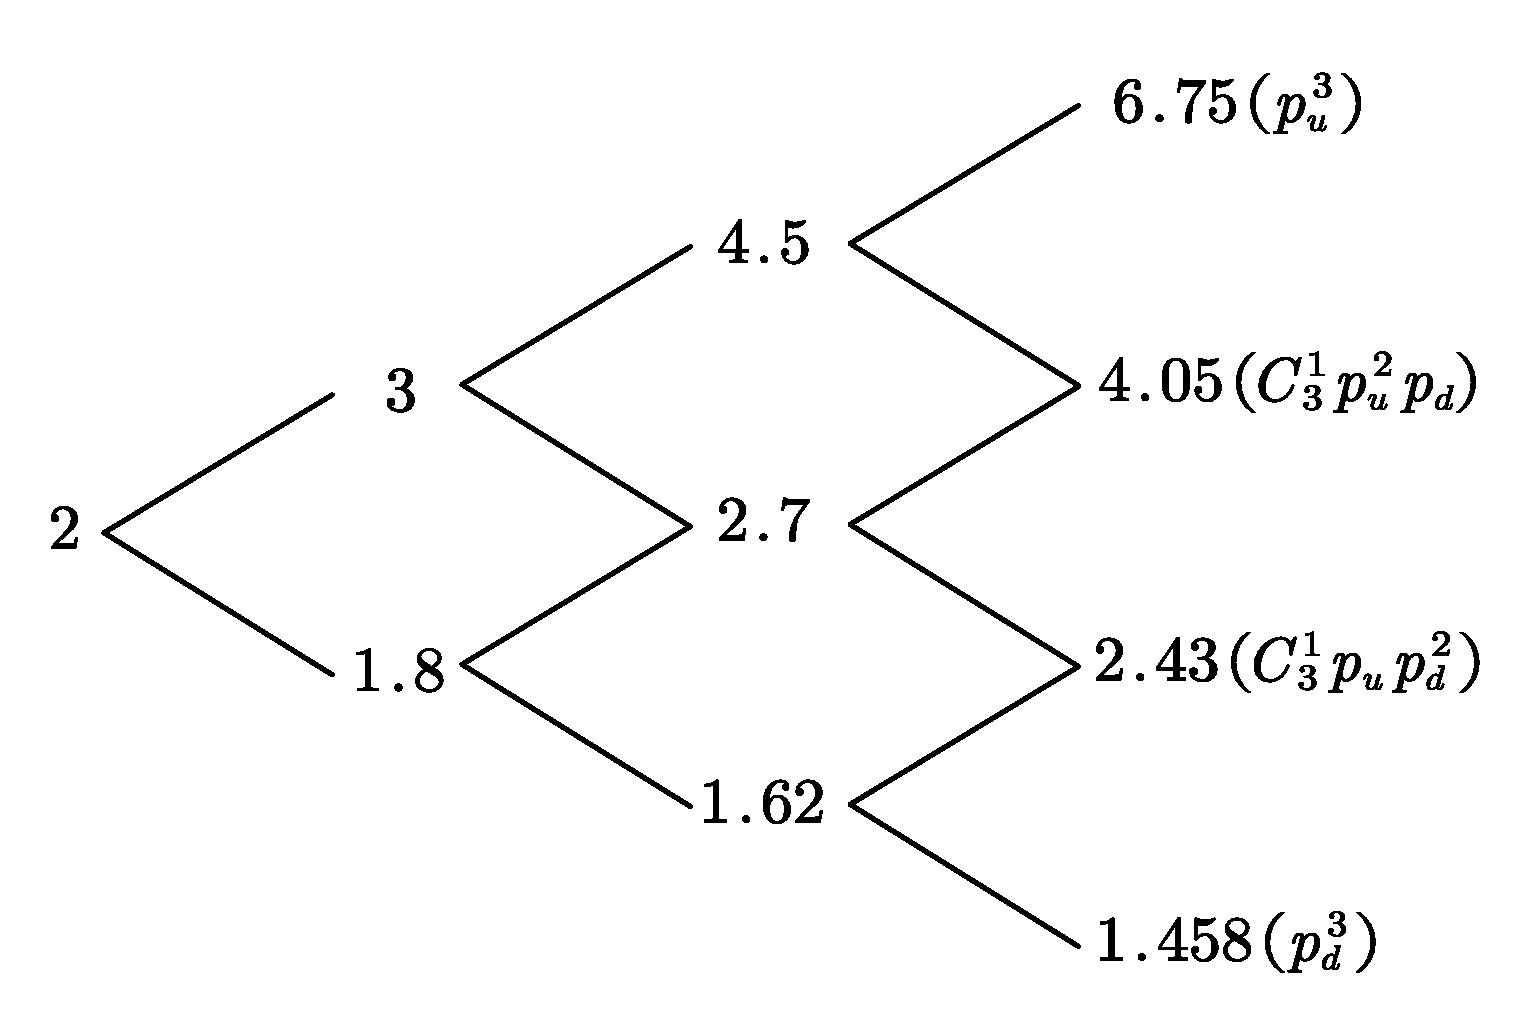
\includegraphics[scale=0.35]{CH3-1-1.pdf}
    \end{center}
    所以,
    \[\mathbb{E} = 6.75\times\left(\frac{1}{3}\right)^3 + 4.05\times3\times\left(\frac{1}{3}\right)^2\times\left(\frac{2}{3}\right)+2.43\times3\times\left(\frac{1}{3}\right)\times\left(\frac{2}{3}\right)^2 + 1.458\times\left(\frac{2}{3}\right)^3 = 2.662\]
    \item \sol\\
    因为
    \[E(S_2) = S_0 (pu+qd)^2 = 1.04^2S_0=27.15 \Rightarrow S_0 = 25.10\]
    所以
    \[S_1 = [30.12, 20.08], S_2 = [36.14,24.10,16.06]\]
    \item \sol\\
    这就是二叉树模型和折现法的应用,同时$pu+(1-p)d=1$.
\end{enumerate}
\subsection{用二叉树模型进行看涨期权定价}
\begin{enumerate}
    \item \sol\\
    先计算$q$:
    \[q = \frac{\e^{r\tau}S_0 - S_d}{S_u - S_d} = \frac{\e^{0.06}\times 120-0.8\times120}{1.7\times120-0.8\times120}=0.2909,\]
    股票的二叉树模型为:
    \begin{center}
        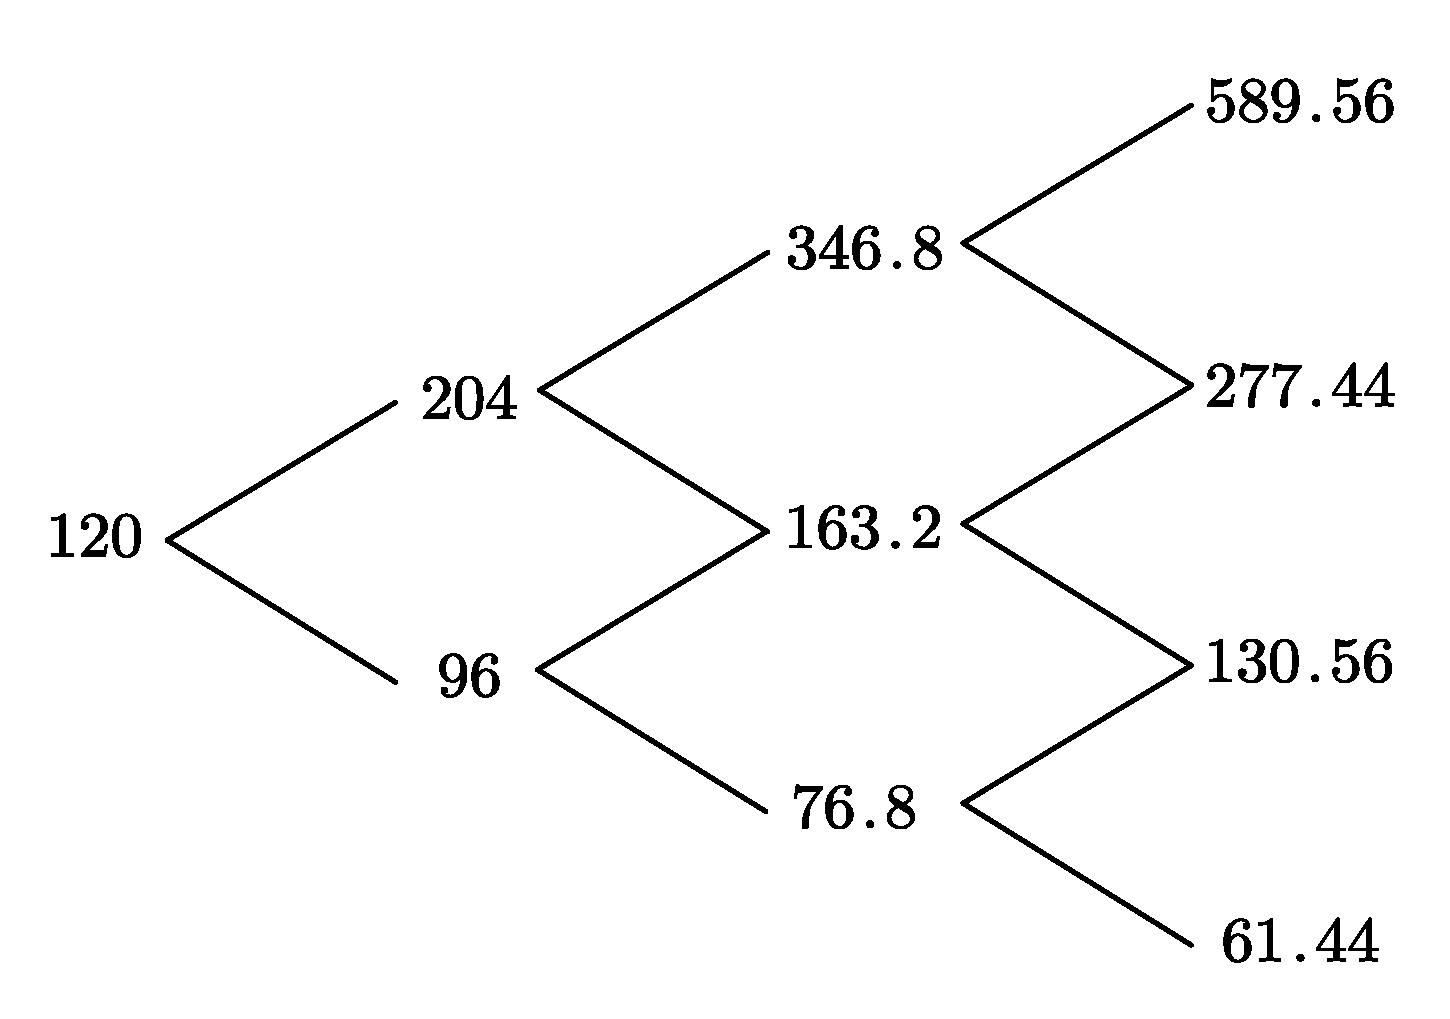
\includegraphics[scale=0.35]{CH3-2-1-股票.pdf}
    \end{center}
    利用
    \[x = \e^{-r\tau}[qa+(1-q)b]=\e^{-0.06}[0.2909a+(1-0.2909)b],\]
    可得期权的二叉树模型为:
    \begin{center}
        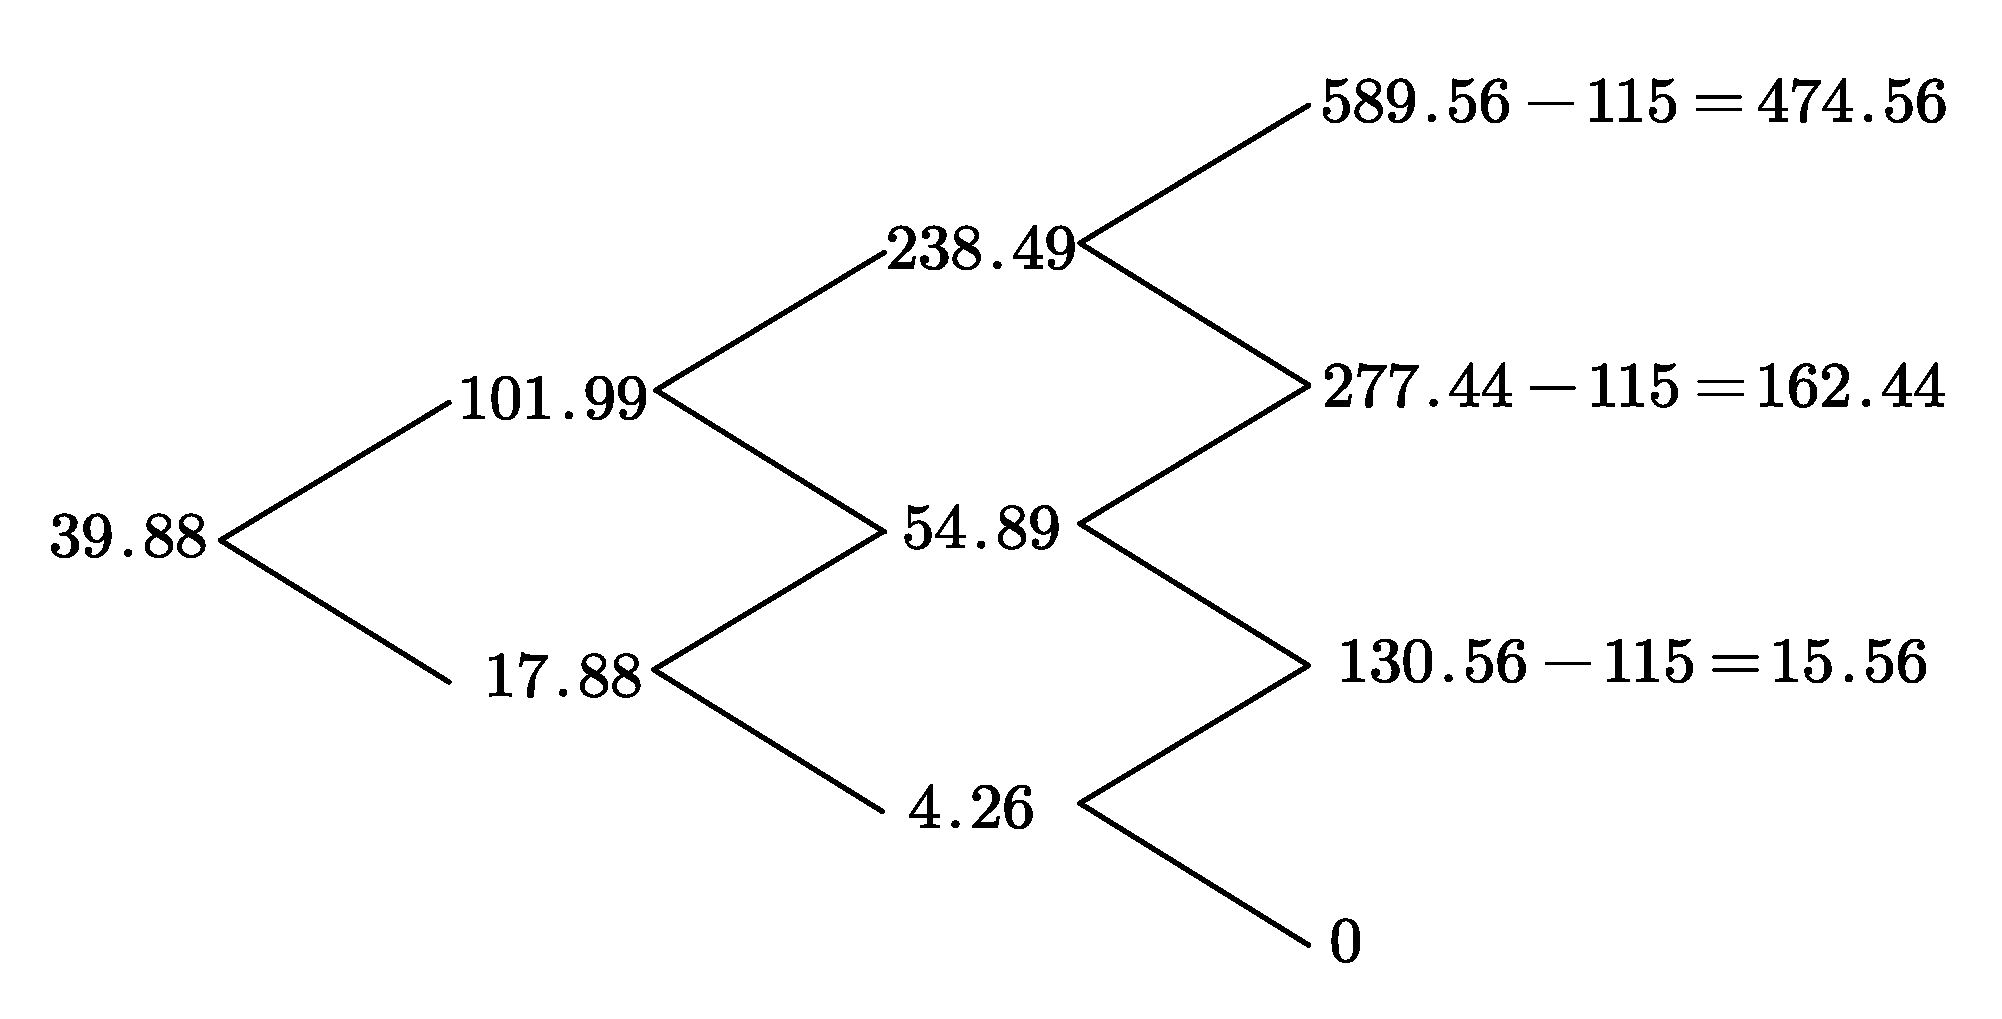
\includegraphics[scale=0.35]{CH3-2-1-期权.pdf}
    \end{center}
    所以在$t=0$时该期权的价格为39.88美元.
    \item \sol\\
    股票二叉树模型同上一题,期权的二叉树模型为:
    \begin{center}
        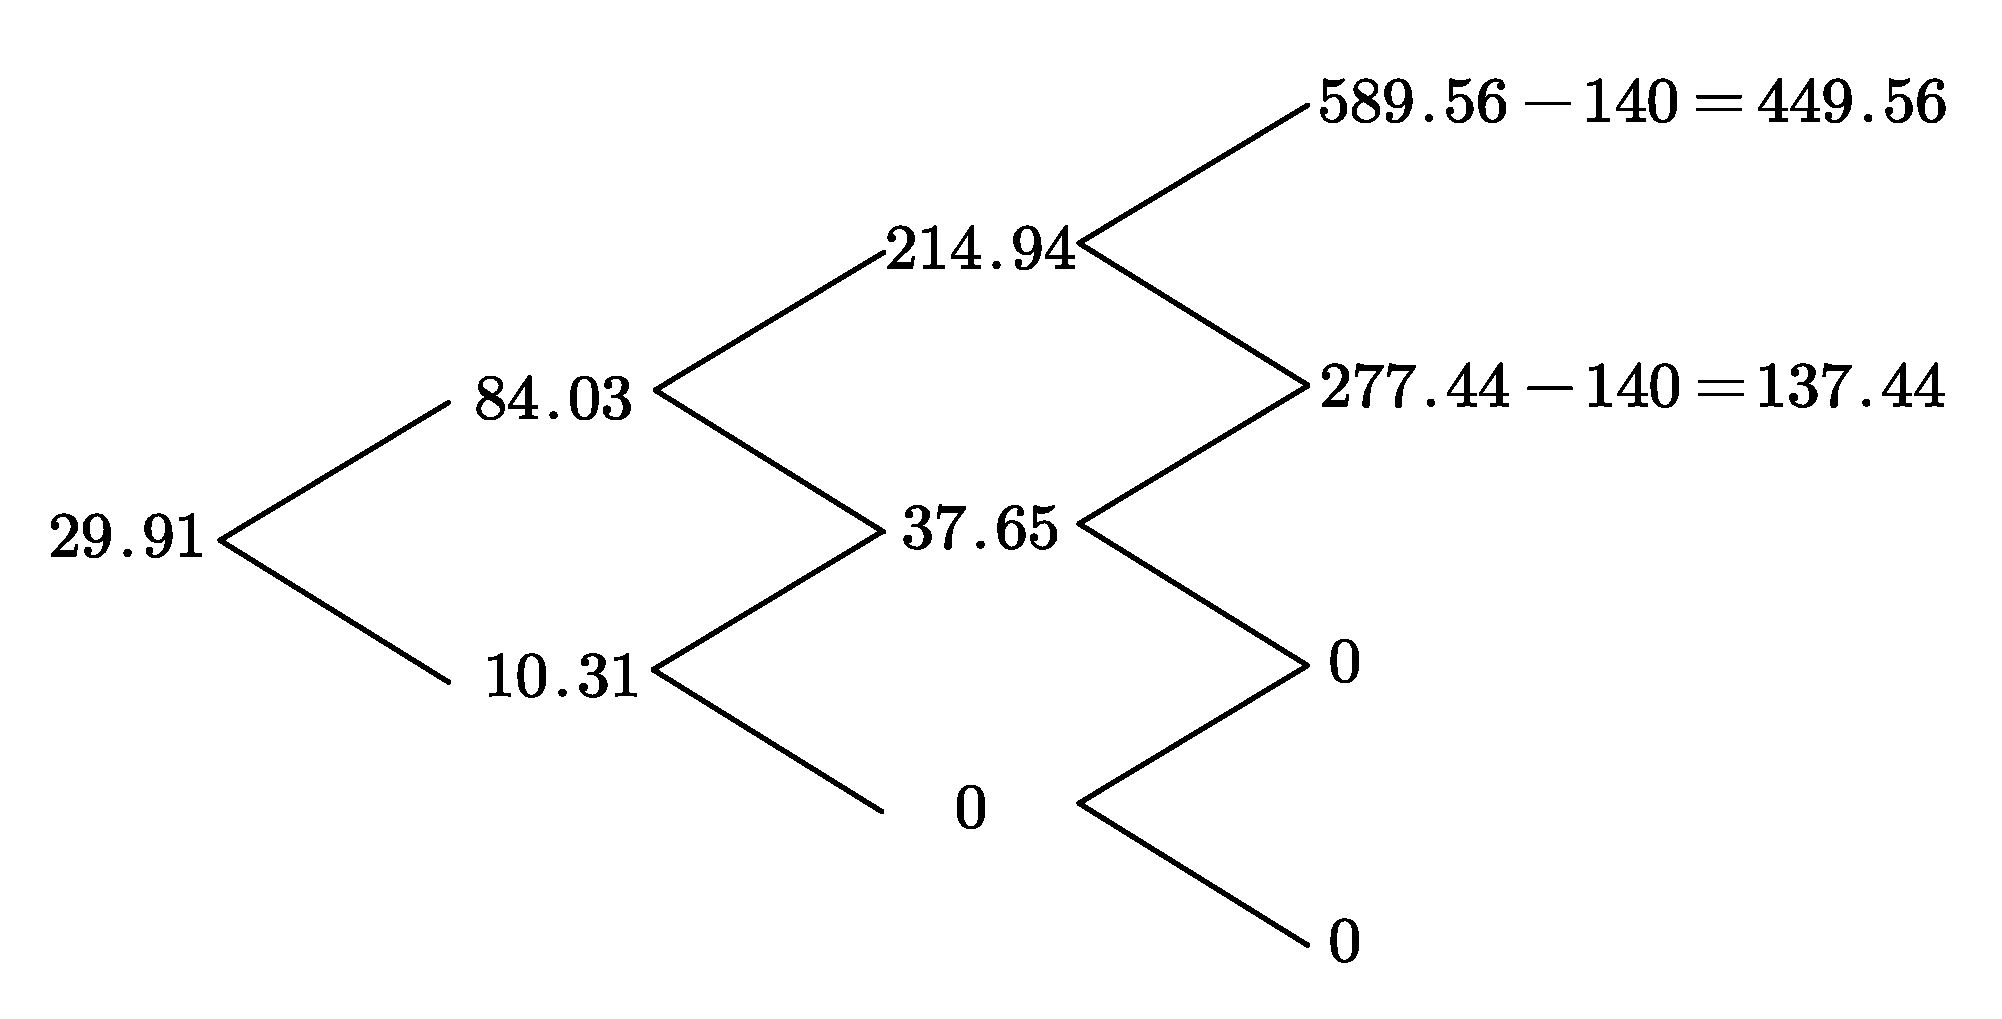
\includegraphics[scale=0.35]{CH3-2-2-期权.pdf}
    \end{center}
    所以在$t=0$时该期权的价格为29.91美元.
    \item \sol\\
    期权的二叉树为:
    \begin{align*}
        V_4 & = [236,  44,   0,   0,   0];\\
        V_3 & = [109.90,  16.06,   0,   0];\\
        V_2 & = [48.79,  5.86,  0];\\
        V_1 & = [20.98,  2.14];\\
        V_0 & = 8.81
    \end{align*}
    所以在$t=0$时该期权的价格为8.81美元.
    \item \omitted
\end{enumerate}
\subsection{美式期权定价}
\begin{enumerate}
    \item \sol\\
    见下表:
    \begin{table}[H]
        \centering
        \begin{tabular}{|c|c|c|c|c|c|c|c|}
            \hline
            期权序号 & (a) & (b) & (c) & (d) & (e) & (f) & (g) \\ \hline
            价格 & 14.79 & 7.40 & 12.26 & 11.54 & 9.04 & 42.02 & 27.84 \\ \hline
        \end{tabular}
    \end{table}
    \item \sol\\
    见下表:
    \begin{table}[H]
        \centering
        \begin{tabular}{|c|c|c|c|c|c|c|c|}
            \hline
            期权序号 & (a) & (b) & (c) & (d) & (e) & (f) & (g) \\ \hline
            价格 & 0.75 & 16.09 & 11.25 & 1.45 & 1.79 & 20.91 & 3.33 \\ \hline
        \end{tabular}
    \end{table}
    \item \sol\\
    见下表:
    \begin{table}[H]
        \centering
        \begin{tabular}{|c|c|c|c|c|c|c|c|}
            \hline
            期权序号 & (a) & (b) & (c) & (d) & (e) & (f) & (g) \\ \hline
            价格 & 1.16 & 20.00 & 15.59 & 1.67 & 2.96 & 26.11 & 3.97 \\ \hline
        \end{tabular}
    \end{table}
    \item \pro\\
    即证美式看跌期权的价格高于欧式看跌期权的价格,而
    \begin{align*}
        V_{eu} & = \frac{0.8\times(110-X) + 0.2 \times 0}{1.06} = 0.7547(110-X)\\
        V_{am} & = \max\left\{V_{eu}, \max(100 - X, 0)\right\} = \max\left\{0.7547(110-X), \max(100 - X, 0)\right\}
    \end{align*}
    所以应提前行权.
\end{enumerate}
\subsection{一类奇异期权——敲出期权的定价}
\begin{enumerate}
    \item \sol\\
    先计算$q$:
    \[q = \frac{\e^{r\tau}S_0 - S_d}{S_u - S_d} = \frac{\e^{0.06}\times 70-56}{87.5-56}=0.5819,\]
    利用向下敲出障碍期权的性质和
    \[x = \e^{-r\tau}[qa+(1-q)b]=\e^{-0.06}[0.5819a+(1-0.5819)b],\]
    可得期权的二叉树模型为:
    \begin{center}
        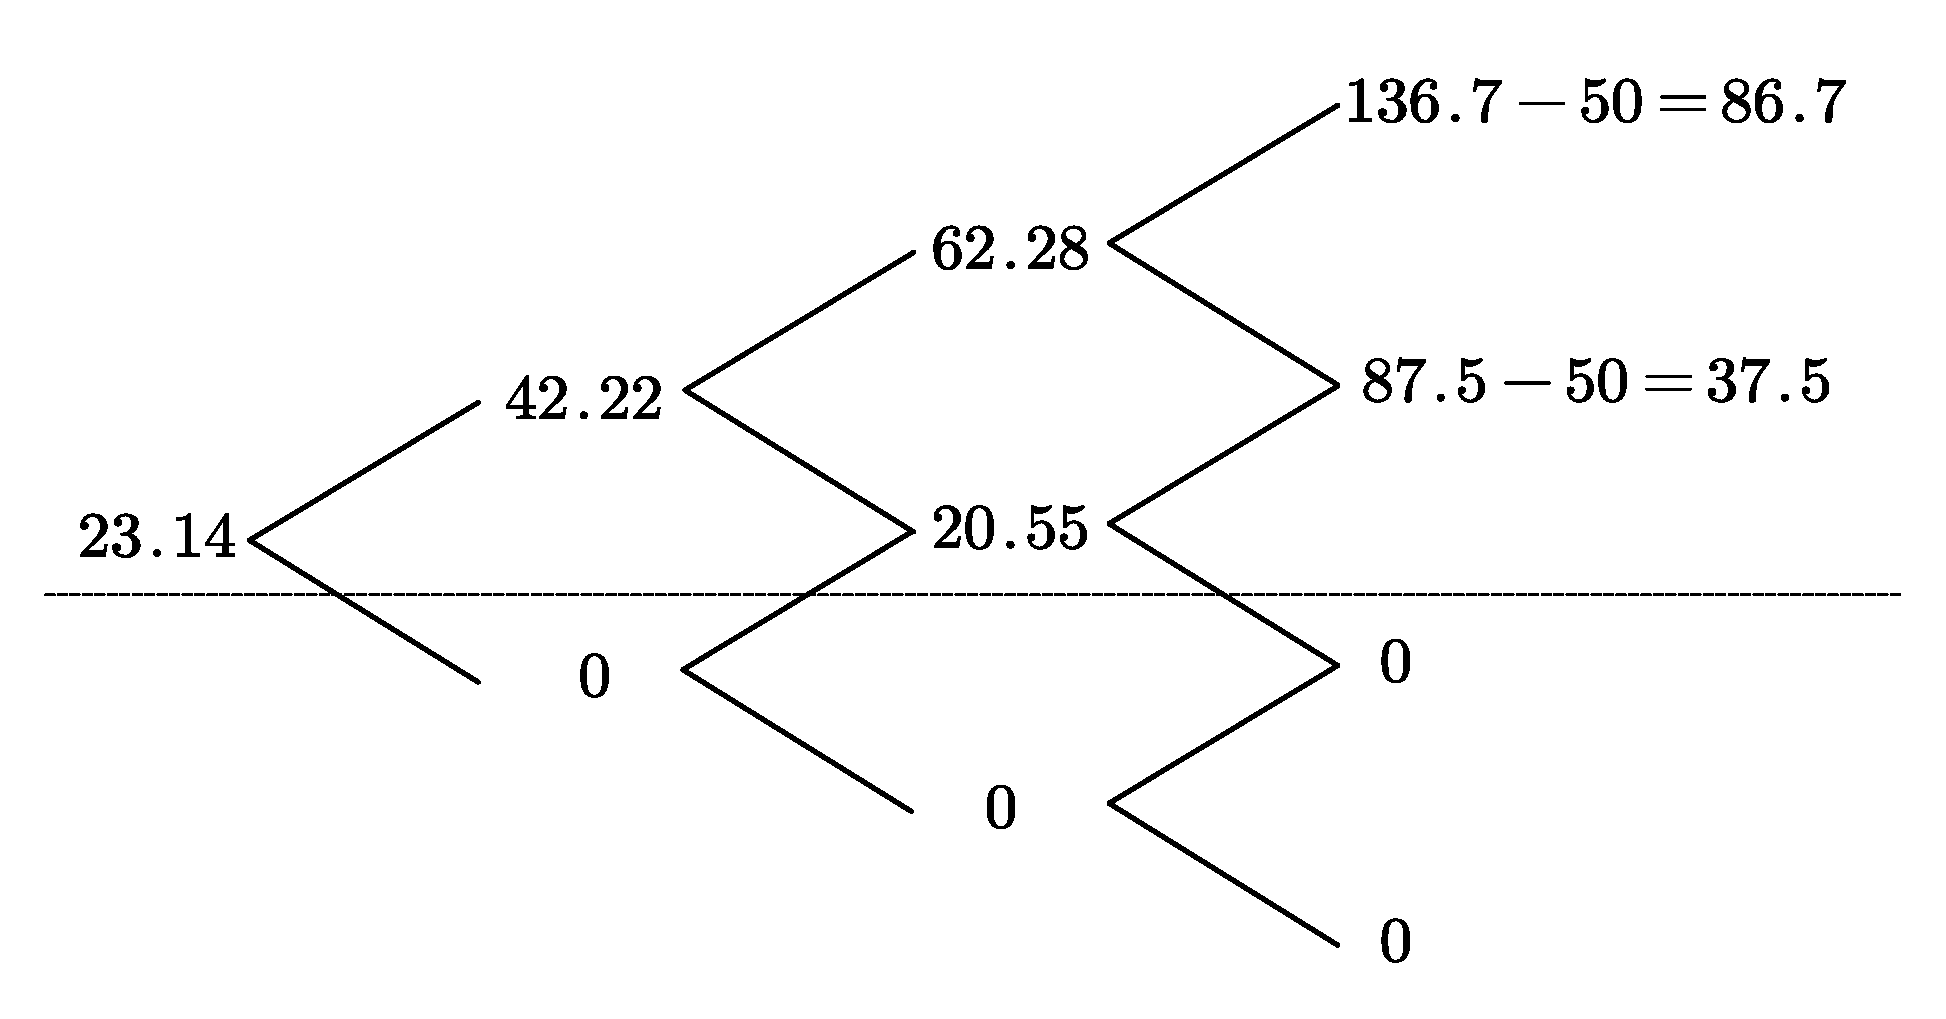
\includegraphics[scale=0.35]{CH3-4-1.pdf}
    \end{center}
    所以$t=0$时刻看涨期权的价格为23.14美元.
    \item \sol\\
    基本数据同上一题,期权的二叉树模型为:
    \begin{center}
        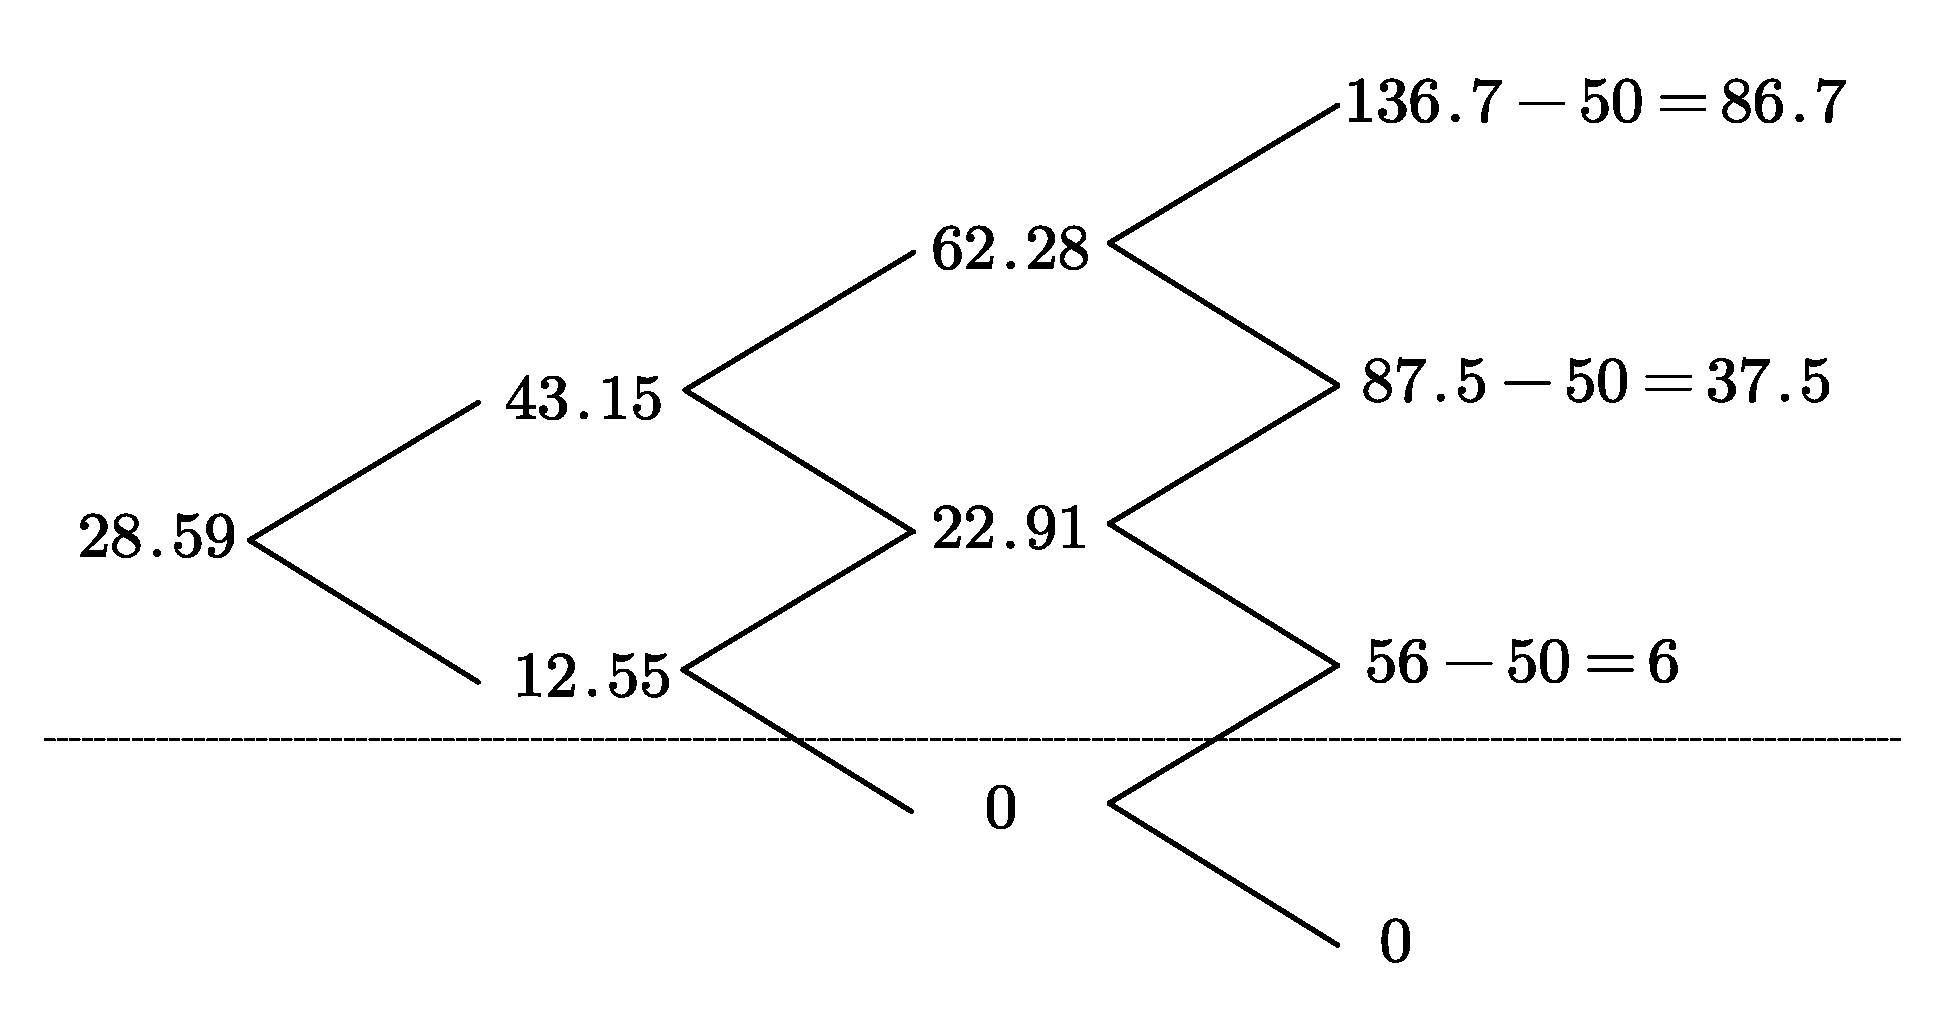
\includegraphics[scale=0.35]{CH3-4-2.pdf}
    \end{center}
    所以$t=0$时刻看涨期权的价格为28.59美元.
    \item \sol\\
    先计算$q$:
    \[q = \frac{\e^{r\tau}S_0 - S_d}{S_u - S_d} = \frac{\e^{0.06}\times 100-90}{110-90}=0.8092,\]
    利用向下敲出障碍期权的性质和
    \[x = \e^{-r\tau}[qa+(1-q)b]=\e^{-0.06}[0.8092a+(1-0.8092)b],\]
    可得期权的二叉树模型为:
    \begin{center}
        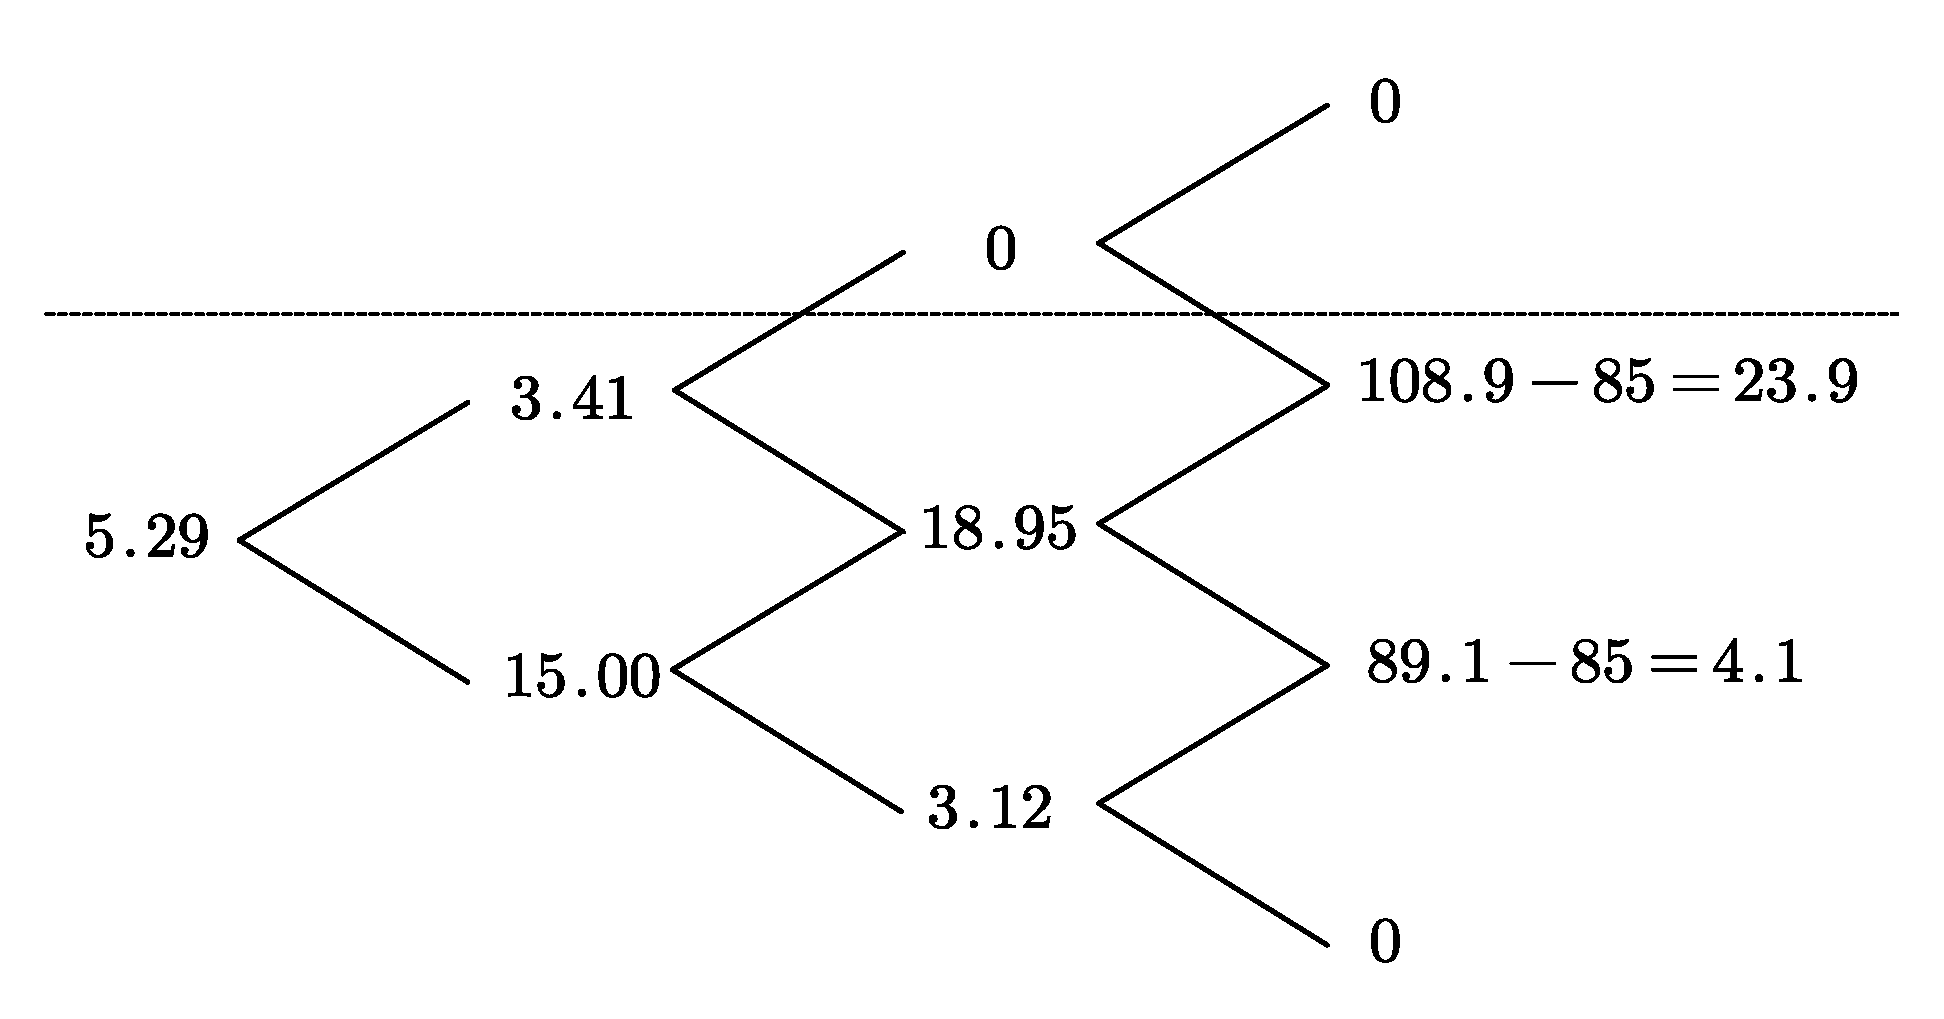
\includegraphics[scale=0.35]{CH3-4-3.pdf}
    \end{center}
    所以$t=0$时刻看涨期权的价格为5.29美元.
\end{enumerate}
\subsection{奇异期权——回望期权定价}
\begin{enumerate}
    \item \sol \textcolor{blue}{使用该节例题中的基本数据}\\
    期权的二叉树为:
    \begin{align*}
        V_2 & = [144, 120, 108, 100];\\
        V_1 & = [127.80, 102.35];\\
        V_0 & = 110.73
    \end{align*}
    所以在$t=0$时该期权的价格为110.73美元.
    \item \sol\\
    具体数据见下表:
    \begin{table}[H]
        \centering
        \begin{tabular}{|c|c|c|}
            \hline
            路径 & 概率 & 最高价 \\ \hline
            $uu$ & $q^2 = 0.1206$ & 144 \\ \hline
            $ud$ & $q(1-q) = 0.2267$ & 120 \\ \hline
            $du$ & $(1-q)q = 0.2267$ & 108 \\ \hline
            $dd$ & $(1-q)^2 = 0.4260$ & 100 \\ \hline
        \end{tabular}
    \end{table}
    所以
    \[E(V_2) = 111.65 \Rightarrow V_0 = E(V_2) \e^{r\tau} = 110.26\]
    所以在$t=0$时该期权的价格为110.26美元.
    \item \sol \textcolor{blue}{使用该节例题中的基本数据}\\
    具体数据见下表:
    \begin{table}[H]
        \centering
        \begin{tabular}{|c|c|c|}
            \hline
            路径 & 概率 & 最高价 \\ \hline
            $uu$ & $q^2 = 0.1206$ & 78.13 \\ \hline
            $ud$ & $q(1-q) = 0.2267$ & 62.5 \\ \hline
            $du$ & $(1-q)q = 0.2267$ & 50 \\ \hline
            $dd$ & $(1-q)^2 = 0.4260$ & 50 \\ \hline
        \end{tabular}
    \end{table}
    所以
    \[E(V_2) = 56.23 \Rightarrow V_0 = E(V_2) \e^{r\tau} = 55.53\]
    所以在$t=0$时该期权的价格为55.53美元.
\end{enumerate}
\subsection{实证数据下二叉树模型分析}
本节无习题
\subsection{$N$期二叉树模型的定价和对冲风险}
\begin{enumerate}
    \item \sol\\
    对于路径$uuuu$,德尔塔值是0.57,0.69,0.89,1.0. 对于路径$udud$,德尔塔值是0.57,0.69,0. 43,0.64. 对于路线$dudu$,德尔塔值是0.57,0.30,0.43,0.0.
    \item \omitted
    \item \sol\\
    对于路径$uuuu$,德尔塔值是$-0.74$,$-0. 17$,0.0,0.0. 对于路径$dddd$,德尔塔值是$-0.74$,$-0.93$,$-1$,$-1$. 对于路径$dudu$,德尔塔值是$-0.74$,$-0.93$,$-0.75$,$-1$.
\end{enumerate}
\clearpage